\chapter{Protein expression and purification}~\label{appx:protein-purification}

\section{Purification of his-tagged protein with metal affinity column}

Most proteins used in this work contain a C-terminal 6x histidine tag.  These proteins can be purified using a cobalt or nickel affinity column.  Proteins purified with this protocol include all Nup variants (FSFG, FG124, etc.), NTF2, mCherry, and GFP.  This protocol is designed for the purification of one 0.5-L cell pellet.  If running more than one column at once, adjust the total buffer volumes accordingly.

This protocol is used for all Nup variants.  For FSFG variants, use the urea concentrations noted in the buffer table.  For FG124 purifications, use 7M guanidine hydrochloride in all buffers (including elution) instead of urea.  Always make urea and guanidine hydrochloride solutions the same day they will be used. \textbf{Do not use urea, guanidine hydrochloride, or other denaturants when purifying ordered proteins.}

To prevent aggregation, BME must be used for any protein that has been labeled with two cysteines. \textbf{Do not use BME if not necessary; any BME solutions must be disposed of as hazardous waste.}

Add the protease inhibitor cocktail (PIC) stock in DMSO immediately before using the buffer.  PIC has a lifetime of about 30 minutes in aqueous solution.  Store all buffers on ice before use.  Incubations should be done at 4$^\circ$C, but the column can be used at room temperature.

\begin{figure}[t!]
\caption[Buffers for metal affinity column purifications.]{Buffer guide for cobalt or nickel affinity column purifications.}
\centering
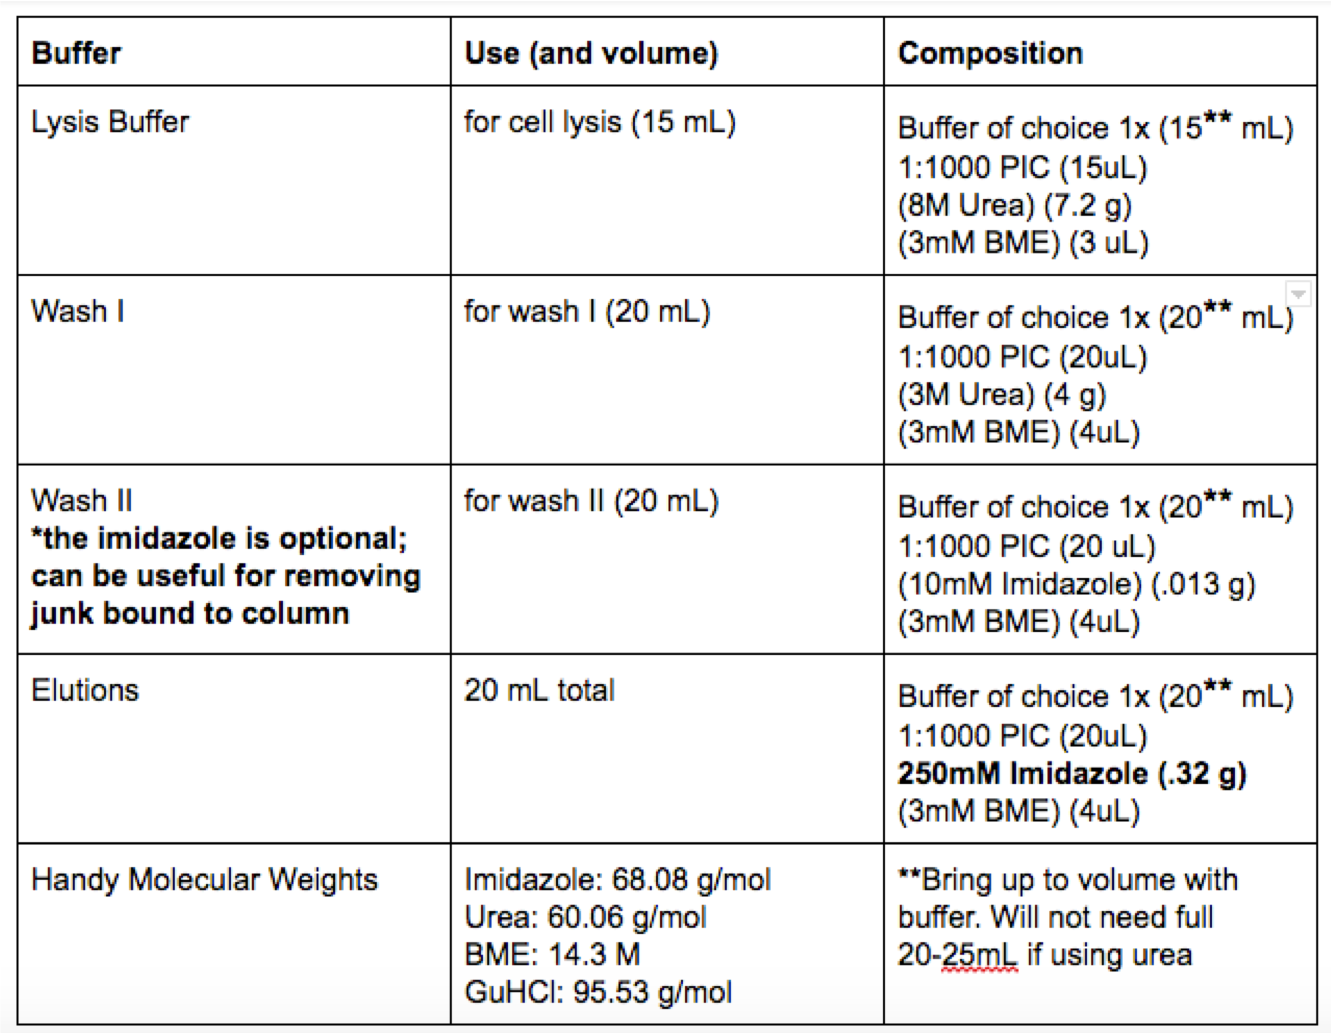
\includegraphics[width=0.8\textwidth]{figs/apps/TALON-table}
\label{fig:TALON-table}
\end{figure}
\begin{enumerate}
\item Remove the periplasmic matrix, if not already done (Sec.~\ref{sec:ppmr}).

\item Lyse the cells. Add 15 mL of lysis buffer to thawed 0.5-L pellet. Resuspend pellet by pipetting up and down or vortexing and then lyse with Qsonica sonicator.  Keep solution on ice. Sonicate for at least two minutes total, in 30 s on, 59 s off pulses.  Power delivered to sample should be at least 20 W.  Centrifuge resulting lysate for at least 15 mins on top speed of Marathon centrifuge to pellet cellular debris.
 
\item Prepare the metal-affinity column.  Gently resuspend the resin into a slurry by slowly turning the bottle.  The beads will be crushed if shaken vigorously. Into a disposable plastic column, pipette enough slurry to contain 3.5-4 mL of beads once the storage buffer has drained out (typically 6-8 mL of slurry, if beads and buffer are stored in a one-to-one mixture).  Equilibrate the column by running 5-10x the bed volume (25-50 mL) of buffer through the column.  Do not let the column run dry at any point in the purification.
 
\item Add supernatant to column and nutate for one hour at 4$^\circ$C.

\item Drain the column. Add wash I buffer and nutate at 4$^\circ$C for 10 minutes.

\item Drain the column. Add wash II buffer, nutate at 4$^\circ$C for 10 minutes, and drain.

\item Elute and collect the protein.  Three elution methods can be used:
\begin{enumerate}
\item \textit{Fractional elution:} Prepare a row of eppendorfs.  Add 5-10 mL elution buffer to open column and catch the draining liquid in fractions with 0.5-1.0 mL (8-16 drops) per eppendorf.  Do not let the column dry.  After all elutions are completed, use the Bradford test to pool the fractions with similar protein concentrations.  \textbf{The Bradford test is unreliable for Nup variants and batch elution should be used.} Fractional elution gives the highest protein concentration and should be used where possible.
\item \textit{Batch elution:} Add a bed volume of elution buffer to column and let drain to remove waste buffer from column.  Watch resin color change carefully so as not to lose protein.  Add 3-5 mL of elution buffer and collect flow-through.
\item \textit{Nutated elution:} Add 5-10 mL of elution buffer to sealed column and nutate for 10-30 minutes.  Collect flow-through.
\end{enumerate}

Early elutions should be fractional or batch elutions.

9) Clean and store the column. Run 5 bed volumes of 20 mM MES hydrate, 300 mM NaCl, pH 5 buffer through the column, then 5 bed volumes DI water.  Store 1:1 in 20\% ethanol.

\end{enumerate}

\section{Periplasmic matrix removal (PPMR)}
\label{sec:ppmr}

The periplasmic matrix (PPM) contains proteases and debris that bind to metal affinity columns.  Removing the PPM before protein purification significantly increases the yield of his-tagged disordered proteins.

\textbf{Note:} Keep both solutions on ice.  Resuspension of pellets should be done by gently pipetting up and down and swirling the tubes.  Do not vortex to resuspend.  Rough treatment of the cells may lyse them.

\begin{enumerate}

\item Spin down cell culture at 4000g (Sorvall centrifuge, GSA rotor) for 10 minutes at 4$^\circ$C.

\item Resuspend pellets in at least 50 mL cold SHE buffer (20\% sucrose, 50mM HEPES, 1mM EDTA pH 7.9) per liter of culture.  Keep tubes on ice.

\item Spin down for 10 minutes at 4000g at 4$^\circ$C.

\item Resuspend pellets in at least 50 mL cold 5mM MgSO$_4$ per liter of culture.

\item Incubate tubes on ice for 10 minutes.

\item Spin down for 10 minutes at 2500g at 4$^\circ$C.

\item Proceed to purification or flash-freeze tubes in liquid nitrogen and store in ultra-low freezer.
\end{enumerate}

\section{Lyophilization}

Lyophilization refers to freeze-drying proteins.  It's a good way to store a known mass of protein before resuspension in hydrogel precursor solution.  All lyophilization in this work was done using a Labconco freeze dry system.  Lyophilization concentrates any salts in the sample buffer.  Therefore, whenever possible, a decomposing buffer should be used.  A 25 mM ammonium bicarbonate buffer was used for all lyophilized Nup variants.  This buffer decomposes into carbon dioxide, ammonia, and water when lyophilized or above 36$^\circ$C.

\begin{enumerate}
\item Dialyze sample into 25 mM ammonium bicarbonate if possible.
\item Perform a BCA to quantify the protein concentration in the sample.  Prepare eppendorf aliquots that contain the desired mass of protein (usually 100 or 200 $\mu$g).
\item Cover the aliquots with parafilm and use a needle to punch a hole in the covering.
\item Flash-freeze the aliquots.
\item Follow lyophilizer instructions.  Keep samples frozen and load as quickly as possible to avoid thawing.  Ensure that the vacuum is below $50 \times 10^{-3}$ mBar.
\item Leave aliquots on lyophilizer at least 12 hours.
\item Remove aliquots from lyophilizer. Remove parafilm and close eppendorfs. Store with desiccant in ultra-low freezer.
\end{enumerate}


